\documentclass[a4paper]{memoir}

\usepackage{tikz,amsmath,amssymb,bm,color}
\usetikzlibrary{calc,arrows,shapes.geometric}

\begin{document}

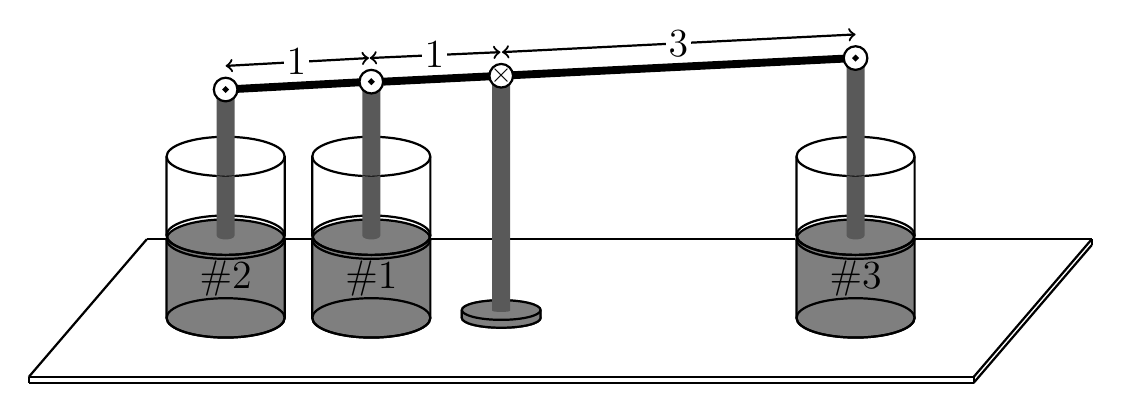
\begin{tikzpicture}[thick,scale=0.5]
\tikzstyle{ann} = [fill=white,font=\footnotesize,inner sep=1pt]
%draw axes

%\draw[ultra thick] (-10,0) -- (10,0);

%\draw[ultra thick] (0,-10) -- (0,10);

%\draw[ultra thick] (0,0) circle (.125);

% rotation axis
% \draw[ultra thick, ->] (0,-2) ++ (-50:.75) arc (-50:300:.75 and .25);
% \draw[ultra thick] (0,-3) node[below] {Rotation axis} -- ++(0,1.5);
% \draw[ultra thick,dashed] (0,-1.5) -- ++(0,4.5);

%%%%%%
\draw (-5,-2.5) -- (-2,1);
\draw (-2,1) -- (-1.5,1);
\draw (1.52,1) -- (2.2,1);
\draw (5.22,1) -- (14.47,1);
\draw (17.49,1) -- (22,1);
\draw (-5,-2.5) -- (19,-2.5);
\draw (19,-2.5) -- (22,1);
%%
\draw (-5,-2.5) -- (-5,-2.65);
\draw (-5,-2.65) -- (19,-2.65);
\draw (19,-2.65) -- (19,-2.5);
\draw (22,1) -- (22,0.85);
\draw (19,-2.65) -- (22,0.85);

%%%%%% Linhas
\draw[line width=1mm] (0,4.8) -- (3.7,5);
\draw[line width=1mm] (4,5) -- (16,5.6);

\draw[arrows=<->] (0,5.4) -- (3.64,5.6);
\node[ann] at (1.8,5.5) {\Large $1$};

\draw[arrows=<->] (3.66,5.6) -- (6.98,5.75);
\node[ann] at (5.3,5.675) {\Large $1$};

\draw[arrows=<->] (7.02,5.75) -- (16,6.2);
\node[ann] at (11.5,5.975) {\Large $3$};

%%%%%% Haste
\draw (7,-1) circle (1 and .25);
\filldraw[gray] (6,-1) arc (-180:0:1 and .25) -- ++(0,.2) arc (0:180:1 and .25) -- cycle;
\draw (6,-1) arc (-180:0:1 and .25) -- ++(0,.2) arc (0:180:1 and .25) -- cycle;
\draw (6,-0.8) arc (-180:0:1 and .25);
\filldraw[black!65,fill opacity=1] (6.8,-0.8) arc (-180:0:0.2 and .02) -- ++(0,6) arc (0:180:0.2 and .02) -- cycle;
\filldraw[draw=black,fill=white] (7,5.15) circle (.3 and .3);
\node at (7,5.15) {$\times$};

%%%%%% Pistão #1
%Cilindro #1
\draw (3.7,-1) circle (1.5 and .5);
\fill[semitransparent] (2.2,-1) arc (-180:0:1.5 and .5) -- ++(0,2) arc (0:180:1.5 and .5) -- cycle;
\draw (2.2,-1) arc (-180:0:1.5 and .5) -- ++(0,2) arc (0:180:1.5 and .5) -- cycle;
\draw (2.2,1) arc (-180:0:1.5 and .5);
\draw (3.7,1.1) circle (1.5 and .5);
%\fill[semitransparent] (2.5,1.1) arc (-180:0:1.5 and .5) -- ++(0,2) arc (0:180:1.5 and .5) -- cycle;
\draw (2.2,1.1) arc (-180:0:1.5 and .5) -- ++(0,2) arc (0:180:1.5 and .5) -- cycle;
\draw (2.2,3.1) arc (-180:0:1.5 and .5);
\node at (3.7,0) {\Large\#1};

%%%%%%% Haste Pistão #1
%Interno
\filldraw[black!65,fill opacity=1](3.5,1.1) arc (-180:0:0.2 and .08) -- ++(0,1.48) arc (0:-180:.2 and .019) -- cycle;
%Externo
\filldraw[black!65,fill opacity=1] (3.5,2.658) arc (-180:0:0.2 and .02) -- ++(0,2.3) arc (0:180:0.2 and .02) -- cycle;
%
\filldraw[draw=black,fill=white] (3.7,5) circle (.3 and .3);
\filldraw[black] (3.7,5) circle (.05 and .05);
%%%%%%%%%%%%%%%%%%%%%%%%%%%%%

%%%%%% Pistão #2
% Cilindro #2
\draw (0,-1) circle (1.5 and .5);
\fill[semitransparent] (-1.5,-1) arc (-180:0:1.5 and .5) -- ++(0,2) arc (0:180:1.5 and .5) -- cycle;
\draw (-1.5,-1) arc (-180:0:1.5 and .5) -- ++(0,2) arc (0:180:1.5 and .5) -- cycle;
\draw (-1.5,1) arc (-180:0:1.5 and .5);
\draw (0,1.1) circle (1.5 and .5);
%\fill[semitransparent] (-1.5,1.1) arc (-180:0:1.5 and .5) -- ++(0,2) arc (0:180:1.5 and .5) -- cycle;
\draw (-1.5,1.1) arc (-180:0:1.5 and .5) -- ++(0,2) arc (0:180:1.5 and .5) -- cycle;
\draw (-1.5,3.1) arc (-180:0:1.5 and .5);
\node at (0,0) {\Large\#2};

%%%% Haste Pistão #2
%Interno
\filldraw[black!65,fill opacity=1](-0.2,1.1) arc (-180:0:0.2 and .08) -- ++(0,1.48) arc (0:-180:.2 and .019) -- cycle;
%Externo
\filldraw[black!65,fill opacity=1] (-0.2,2.658) arc (-180:0:0.2 and .02) -- ++(0,2.1) arc (0:180:0.2 and .02) -- cycle;
%
\filldraw[draw=black,fill=white] (0,4.8) circle (.3 and .3);
\filldraw[black] (0,4.8) circle (.05 and .05);
%%%%%%%%%%%%%%%%%%%%%%%%%%

%%%%%%%
%Cilindro #3
\draw (16,-1) circle (1.5 and .5);
\fill[semitransparent] (14.5,-1) arc (-180:0:1.5 and .5) -- ++(0,2) arc (0:180:1.5 and .5) -- cycle;
\draw (14.5,-1) arc (-180:0:1.5 and .5) -- ++(0,2) arc (0:180:1.5 and .5) -- cycle;
\draw (14.5,1) arc (-180:0:1.5 and .5);
\draw (16,1.1) circle (1.5 and .5);
%\fill[semitransparent] (14.5,1.1) arc (-180:0:1.5 and .5) -- ++(0,2) arc (0:180:1.5 and .5) -- cycle;
\draw (14.5,1.1) arc (-180:0:1.5 and .5) -- ++(0,2) arc (0:180:1.5 and .5) -- cycle;
\draw (14.5,3.1) arc (-180:0:1.5 and .5);
\node at (16,0) {\Large\#3};

%%%% Haste Pistão #3
%Interno
\filldraw[black!65,fill opacity=1](15.8,1.1) arc (-180:0:0.2 and .08) -- ++(0,1.48) arc (0:-180:.2 and .019) -- cycle;
%Externo
\filldraw[black!65,fill opacity=1] (15.8,2.658) arc (-180:0:0.2 and .02) -- ++(0,2.75) arc (0:180:0.2 and .02) -- cycle;
%
\filldraw[draw=black,fill=white] (16,5.6) circle (.3 and .3);
\filldraw[black] (16,5.6) circle (.05 and .05);
%%%%%%%%%%%%%%%%%%%%%%%%%%
\end{tikzpicture}

\end{document}
